\chapter{Probabilistic computation}\label{randomizedalgchap}

\begin{objectives} \label[objectives]{See-examples-of-randomize}

\begin{itemize}
\tightlist
\item
  See examples of randomized algorithms\\
\item
  Get more comfort with analyzing probabilistic processes and tail
  bounds\\
\item
  Success amplification using tail bounds\\
\end{itemize}

\end{objectives}

\begin{quote}
\emph{``in 1946 .. (I asked myself) what are the chances that a Canfield
solitaire laid out with 52 cards will come out successfully? After
spending a lot of time trying to estimate them by pure combinatorial
calculations, I wondered whether a more practical method \ldots{} might
not be to lay it our say one hundred times and simple observe and
count''}, Stanislaw Ulam, 1983
\end{quote}

\begin{quote}
\emph{``The salient features of our method are that it is probabilistic
\ldots{} and with a controllable miniscule probability of error.''},
Michael Rabin, 1977
\end{quote}

In early computer systems, much effort was taken to drive \emph{out}
randomness and noise. Hardware components were prone to
non-deterministic behavior from a number of causes, whether it was
vacuum tubes overheating or actual physical bugs causing short circuits
(see \cref{bugfig}). This motivated John von Neumann, one of the early
computing pioneers, to write a paper on how to \emph{error correct}
computation, introducing the notion of \emph{redundancy}.


\begin{marginfigure}
\centering
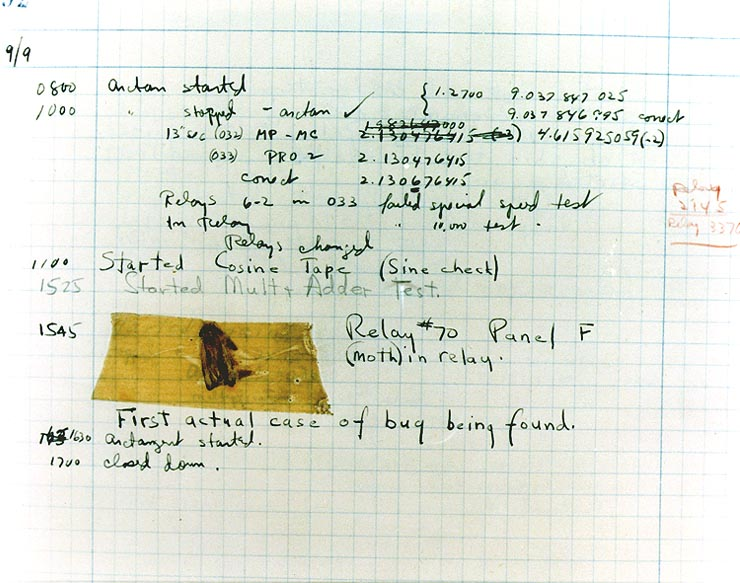
\includegraphics[width=\linewidth, height=1.5in, keepaspectratio]{../figure/bug.jpg}
\caption{A 1947 entry in the
\href{http://americanhistory.si.edu/collections/search/object/nmah_334663}{log
book} of the Harvard MARK II computer containing an actual bug that
caused a hardware malfunction. By Courtesy of the Naval Surface Warfare
Center.}
\label{bugfig}
\end{marginfigure}

So it is quite surprising that randomness turned out not just a
hindrance but also a \emph{resource} for computation, enabling us to
achieve tasks much more efficiently than previously known. One of the
first applications involved the very same John von Neumann. While he was
sick in bed and playing cards, Stan Ulam came up with the observation
that calculating statistics of a system could be done much faster by
running several randomized simulations. He mentioned this idea to von
Neumann, who became very excited about it; indeed, it turned out to be
crucial for the neutron transport calculations that were needed for
development of the Atom bomb and later on the hydrogen bomb. Because
this project was highly classified, Ulam, von Neumann and their
collaborators came up with the codeword ``Monte Carlo'' for this
approach (based on the famous casinos where Ulam's uncle gambled). The
name stuck, and randomized algorithms are known as Monte Carlo
algorithms to this day.\footnote{Some texts also talk about ``Las Vegas
  algorithms'' that always return the right answer but whose running
  time is only polynomial on the average. Since this Monte Carlo vs Las
  Vegas terminology is confusing, we will not use these terms anymore,
  and simply talk about randomized algorithms.}

In this chapter, we will see some examples of randomized algorithms that
use randomness to compute a quantity in a faster or simpler way than was
known otherwise. We will describe the algorithms in an informal /
``pseudo-code'' way, rather than as NAND-TM, NAND-RAM programs or Turing
macines. In \cref{chapmodelrand} we will discuss how to augment the
computational models we say before to incorporate the ability to ``toss
coins''.

\section{Finding approximately good maximum
cuts.}\label{Finding-approximately-goo}

We start with the following example. Recall the \emph{maximum cut
problem} of finding, given a graph \(G=(V,E)\), the cut that maximizes
the number of edges. This problem is \(\mathbf{NP}\)-hard, which means
that we do not know of any efficient algorithm that can solve it, but
randomization enables a simple algorithm that can cut at least half of
the edges:

\hypertarget{maxcutthm}{}
\begin{theorem}[Approximating max cut] \label[theorem]{maxcutthm}

There is an efficient probabilistic algorithm that on input an
\(n\)-vertex \(m\)-edge graph \(G\), outputs a cut \((S,\overline{S})\)
that cuts at least \(m/2\) of the edges of \(G\) in expectation.

\end{theorem}

\begin{proofidea} \label[proofidea]{We-simply-choose-a-random}

We simply choose a \emph{random cut}: we choose a subset \(S\) of
vertices by choosing every vertex \(v\) to be a member of \(S\) with
probability \(1/2\) independently. It's not hard to see that each edge
is cut with probability \(1/2\) and so the expected number of cut edges
is \(m/2\).

\end{proofidea}

\begin{proof}[Proof of \cref{maxcutthm}] \label[proof]{The-algorithm-is-extremel}

The algorithm is extremely simple:

\begin{quote} \label[quote]{Algorithm-Random-CutInput}

\textbf{Algorithm Random Cut:}

\textbf{Input:} Graph \(G=(V,E)\) with \(n\) vertices and \(m\) edges.
Denote \(V = \{ v_0,v_1,\ldots, v_{n-1}\}\).

\textbf{Operation:}

\begin{enumerate}
\def\labelenumi{\arabic{enumi}.}
\item
  Pick \(x\) uniformly at random in \(\{0,1\}^n\).
\item
  Let \(S \subseteq V\) be the set
  \(\{ v_i \;:\; x_i = 1 \;,\; i\in [n] \}\) that includes all vertices
  corresponding to coordinates of \(x\) where \(x_i=1\).
\item
  Output the cut \((S,\overline{S})\).
\end{enumerate}

\end{quote}

We claim that the expected number of edges cut by the algorithm is
\(m/2\). Indeed, for every edge \(e \in E\), let \(X_e\) be the random
variable such that \(X_e(x)=1\) if the edge \(e\) is cut by \(x\), and
\(X_e(x)=0\) otherwise. For every such edge \(e =\{ i,j \}\),
\(X_e(x)=1\) if and only if \(x_i \neq x_j\). Since the pair
\((x_i,x_j)\) obtains each of the values \(00,01,10,11\) with
probability \(1/4\), the probability that \(x_i \neq x_j\) is \(1/2\)
and hence \(\E[X_e]=1/2\). If we let \(X\) be the random variable
corresponding to the total number of edges cut by \(S\), then
\(X = \sum_{e\in E} X_e\) and hence by linearity of expectation

\[\E[X] = \sum_{e\in E} \E[X_e] = m(1/2) = m/2 \;.\]

\end{proof}

\paragraph{Randomized algorithms work in the worst case.} It is tempting
of a randomized algorithm such as the one of \cref{maxcutthm} as an
algorithm that works for a ``random input graph'' but it is actually
much better than that. The expectation in this theorem is \emph{not}
taken over the choice of the graph, but rather only over the
\emph{random choices of the algorithm}. In particular, \emph{for every
graph \(G\)}, the algorithm is guaranteed to cut half of the edges of
the input graph in expectation. That is,

\hypertarget{randomworstcaseidea}{}
\begin{bigidea} \label[bigidea]{randomworstcaseidea}

A randomized algorithm outputs the correct value with good probability
on \emph{every possible input}.

\end{bigidea}

We will define more formally what ``good probability'' means in
\cref{chapmodelrand} but the crucial point is that this probability is
always only taken over the random choices of the algorithm, while the
input is \emph{not} chosen at random.

\subsection{Amplifying the success of randomized
algorithms}\label{Amplifying-the-success-of}

\cref{maxcutthm} gives us an algorithm that cuts \(m/2\) edges in
\emph{expectation}. But, as we saw before, expectation does not
immediately imply concentration, and so a priori, it may be the case
that when we run the algorithm, most of the time we don't get a cut
matching the expectation. Luckily, we can \emph{amplify} the probability
of success by repeating the process several times and outputting the
best cut we find. We start by arguing that the probability the algorithm
above succeeds in cutting at least \(m/2\) edges is not \emph{too} tiny.

\hypertarget{cutprob}{}
\begin{lemma} \label[lemma]{cutprob}

The probability that a random cut in an \(m\) edge graph cuts at least
\(m/2\) edges is at least \(1/(2m)\).

\end{lemma}

\begin{proofidea} \label[proofidea]{To-see-the-idea-behind-th}

To see the idea behind the proof, think of the case that \(m=1000\). In
this case one can show that we will cut at least \(500\) edges with
probability at least \(0.001\) (and so in particular larger than
\(1/(2m)=1/2000\)). Specifically, if we assume otherwise, then this
means that with probability more than \(0.999\) the algorithm cuts
\(499\) or fewer edges. But since we can never cut more than the total
of \(1000\) edges, given this assumption, the highest value the expected
number of edges cut is if we cut exactly \(499\) edges with probability
\(0.999\) and cut \(1000\) edges with probability \(0.001\). Yet even in
this case the expected number of edges will be
\(0.999 \cdot 499 + 0.001 \cdot 1000 < 500\), which contradicts the fact
that we've calculated the expectation to be at least \(500\) in
\cref{maxcutthm}.

\end{proofidea}

\begin{proof}[Proof of \cref{cutprob}] \label[proof]{Let-p-be-the-probability-}

Let \(p\) be the probability that we cut at least \(m/2\) edges and
suppose, towards a contradiction, that \(p<1/(2m)\). Since the number of
edges cut is an integer, and \(m/2\) is a multiple of \(0.5\), by
definition of \(p\), with probability \(1-p\) we cut at most
\(m/2 - 0.5\) edges. Moreover, since we can never cut more than \(m\)
edges, under our assumption that \(p<m/2\), we can bound the expected
number of edges cut by

\[
pm + (1-p)(m/2-0.5)  \leq pm + m/2-0.5
\] But if \(p<1/(2m)\) then \(pm<0.5\) and so the righthand side is
smaller than \(m/2\), which contradicts the fact that (as proven in
\cref{maxcutthm}) the expected number of edges cut is at least \(m/2\).

\end{proof}

\subsection{Success amplification}\label{Success-amplification}

\cref{cutprob} shows that our algorithm succeeds at least \emph{some} of
the time, but we'd like to succeed almost \emph{all} of the time. The
approach to do that is to simply \emph{repeat} our algorithm many times,
with fresh randomness each time, and output the best cut we get in one
of these repetitions. It turns out that with extremely high probability
we will get a cut of size at least \(m/2\). For example, if we repeat
this experiment \(2000m\) times, then (using the inequality
\((1-1/k)^k \leq 1/e \leq 1/2\)) we can show that the probability that
we will never cut at least \(m/2\) edges is at most

\[
(1-1/(2m))^{2000 m} \leq 2^{-1000} \;.
\]

More generally, the same calculations can be used to show the following
lemma:

\hypertarget{cutalgorithmamplificationlem}{}
\begin{lemma} \label[lemma]{cutalgorithmamplificationlem}

There is an algorithm that on input a graph \(G=(V,E)\) and a number
\(k\), runs in time polynomial in \(|V|\) and \(k\) and outputs a cut
\((S,\overline{S})\) such that \[
\Pr[ \text{number of edges cut by $(S,\overline{S})$ } \geq |E|/2 ] \geq 1- 2^{-k} \;.
\]

\end{lemma}

\begin{proof}[Proof of \cref{cutalgorithmamplificationlem}] \label[proof]{The-algorithm-will-work-a}

The algorithm will work as follows:

\begin{quote} \label[quote]{Algorithm-AMPLIFY-RANDOM-}

\textbf{Algorithm AMPLIFY RANDOM CUT:}

\textbf{Input:} Graph \(G=(V,E)\) with \(n\) vertices and \(m\) edges.
Denote \(V = \{ v_0,v_1,\ldots, v_{n-1}\}\). Number \(k>0\).

\textbf{Operation:}

\begin{enumerate}
\def\labelenumi{\arabic{enumi}.}
\item
  Repeat the following \(200km\) times:

  \begin{enumerate}
  \def\labelenumii{\alph{enumii}.}
  \item
    Pick \(x\) uniformly at random in \(\{0,1\}^n\).
  \item
    Let \(S \subseteq V\) be the set
    \(\{ v_i \;:\; x_i = 1 \;,\; i\in [n] \}\) that includes all
    vertices corresponding to coordinates of \(x\) where \(x_i=1\).
  \item
    If \((S,\overline{S})\) cuts at least \(m/2\) then halt and output
    \((S,\overline{S})\).
  \end{enumerate}
\item
  Output ``failed''
\end{enumerate}

\end{quote}

We leave completing the analysis as an exercise to the reader (see
\cref{cutalgorithmamplificationlemex}).

\end{proof}

\subsection{Two-sided amplification}\label{Two-sided-amplification}

The analysis above relied on the fact that the maximum cut has \emph{one
sided error}. By this we mean that if we get a cut of size at least
\(m/2\) then we know we have succeeded. This is common for randomized
algorithms, but is not the only case. In particular, consider the task
of computing some Boolean function \(F:\{0,1\}^* \rightarrow \{0,1\}\).
A randomized algorithm \(A\) for computing \(F\), given input \(x\),
might toss coins and succeed in outputting \(F(x)\) with probability,
say, \(0.9\). We say that \(A\) has \emph{two sided errors} if there is
positive probability that \(A(x)\) outputs \(1\) when \(F(x)=0\), and
positive probability that \(A(x)\) outputs \(0\) when \(F(x)=1\). In
such a case, to simplify \(A\)'s success, we cannot simply repeat it
\(k\) times and output \(1\) if a single one of those repetitions
resulted in \(1\), nor can we output \(0\) if a single one of the
repetitions resulted in \(0\). But we can output the \emph{majority
value} of these repetitions. By the Chernoff bound (\cref{chernoffthm}),
with probability \emph{exponentially close} to \(1\) (i.e.,
\(1-2^{\Omega(k)}\)), the fraction of the repetitions where \(A\) will
output \(F(x)\) will be at least, say \(0.89\), and in such cases we
will of course output the correct answer.

The above translates into the following theorem

\hypertarget{amplifyalg}{}
\begin{theorem}[Two-sided amplification] \label[theorem]{amplifyalg}

If \(F:\{0,1\}^* \rightarrow \{0,1\}\) is a function such that there is
a polynomial-time algorithm \(A\) satisfying \[
\Pr[A(x) = F(x)] \geq 0.51
\] for every \(x\in \{0,1\}^*\), then there is a polynomial time
algorithm \(B\) satisfying \[
\Pr[ B(x) = F(x) ] \geq 1 - 2^{-|x|}
\] for every \(x\in \{0,1\}^*\).

\end{theorem}

We omit the proof of \cref{amplifyalg}, since we will prove a more
general result later on in \cref{amplificationthm}.

\subsection{What does this mean?}\label{What-does-this-mean}

We have shown a probabilistic algorithm that on any \(m\) edge graph
\(G\), will output a cut of at least \(m/2\) edges with probability at
least \(1-2^{-1000}\). Does it mean that we can consider this problem as
``easy''? Should we be somewhat wary of using a probabilistic algorithm,
since it can sometimes fail?

First of all, it is important to emphasize that this is still a
\emph{worst case} guarantee. That is, we are not assuming anything about
the \emph{input graph}: the probability is only due to the
\emph{internal randomness of the algorithm}. While a probabilistic
algorithm might not seem as nice as a deterministic algorithm that is
\emph{guaranteed} to give an output, to get a sense of what a failure
probability of \(2^{-1000}\) means, note that:

\begin{itemize}
\item
  The chance of winning the Massachusetts Mega Million lottery is one
  over \((75)^5\cdot 15\) which is roughly \(2^{-35}\). So \(2^{-1000}\)
  corresponds to winning the lottery about \(300\) times in a row, at
  which point you might not care so much about your algorithm failing.
\item
  The chance for a U.S. resident to be struck by lightning is about
  \(1/700000\), which corresponds to about \(2^{-45}\) chance that
  you'll be struck by lightning the very second that you're reading this
  sentence (after which again you might not care so much about the
  algorithm's performance).
\item
  Since the earth is about 5 billion years old, we can estimate the
  chance that an asteroid of the magnitude that caused the dinosaurs'
  extinction will hit us this very second to be about \(2^{-60}\). It is
  quite likely that even a deterministic algorithm will fail if this
  happens.
\end{itemize}

So, in practical terms, a probabilistic algorithm is just as good as a
deterministic one. But it is still a theoretically fascinating question
whether randomized algorithms actually yield more power, or whether is
it the case that for any computational problem that can be solved by
probabilistic algorithm, there is a deterministic algorithm with nearly
the same performance.\footnote{This question does have some significance
  to practice, since hardware that generates high quality randomness at
  speed is nontrivial to construct.} For example, we will see in
\cref{maxcutex} that there is in fact a deterministic algorithm that can
cut at least \(m/2\) edges in an \(m\)-edge graph. We will discuss this
question in generality in \cref{chapmodelrand}. For now, let us see a
couple of examples where randomization leads to algorithms that are
better in some sense than the known deterministic algorithms.

\subsection{Solving SAT through
randomization}\label{Solving-SAT-through-rando}

The 3SAT problem is \(\mathbf{NP}\) hard, and so it is unlikely that it
has a polynomial (or even subexponential) time algorithm. But this does
not mean that we can't do at least somewhat better than the trivial
\(2^n\) algorithm for \(n\)-variable 3SAT. The best known worst-case
algorithms for 3SAT are randomized, and are related to the following
simple algorithm, variants of which are also used in practice:

\begin{quote} \label[quote]{Algorithm-WalkSATInput-An}

\textbf{Algorithm WalkSAT:}

\textbf{Input:} An \(n\) variable 3CNF formula \(\varphi\).

\textbf{Parameters:} \(T,S \in \N\)

\textbf{Operation:}

\begin{enumerate}
\def\labelenumi{\arabic{enumi}.}
\item
  Repeat the following \(T\) steps:

  \begin{enumerate}
  \def\labelenumii{\alph{enumii}.}
  \item
    Choose a random assignment \(x\in \{0,1\}^n\) and repeat the
    following for \(S\) steps:

    \begin{enumerate}
    \def\labelenumiii{\arabic{enumiii}.}
    \item
      If \(x\) satisfies \(\varphi\) then output \(x\).
    \item
      Otherwise, choose a random clause
      \((\ell_i \vee \ell_j \vee \ell_k)\) that \(x\) does not satisfy,
      choose a random literal in \(\ell_i,\ell_j,\ell_k\) and modify
      \(x\) to satisfy this literal.
    \end{enumerate}
  \end{enumerate}
\item
  If all the \(T\cdot S\) repetitions above did not result in a
  satisfying assignment then output \texttt{Unsatisfiable}
\end{enumerate}

\end{quote}

The running time of this algorithm is \(S\cdot T \cdot poly(n)\), and so
the key question is how small we can make \(S\) and \(T\) so that the
probability that WalkSAT outputs \texttt{Unsatisfiable} on a satisfiable
formula \(\varphi\) is small. It is known that we can do so with
\(\ensuremath{\mathit{ST}} = \tilde{O}((4/3)^n) = \tilde{O}(1.333\ldots^n)\)
(see \cref{walksatex} for a weaker result), but we'll show below a
simpler analysis yielding
\(\ensuremath{\mathit{ST}}= \tilde{O}(\sqrt{3}^n) = \tilde{O}(1.74^n)\),
which is still much better than the trivial \(2^n\) bound.\footnote{At
  the time of this writing, the best known
  \href{https://arxiv.org/pdf/1103.2165.pdf}{randomized} algorithms for
  3SAT run in time roughly \(O(1.308^n)\), and the best known
  \href{https://arxiv.org/pdf/1102.3766v1.pdf}{deterministic} algorithms
  run in time \(O(1.3303^n)\) in the worst case.}

\hypertarget{walksatthm}{}
\begin{theorem}[WalkSAT simple analysis] \label[theorem]{walksatthm}

If we set \(T=100\cdot \sqrt{3}^{n}\) and \(S= n/2\), then the
probability we output \texttt{Unsatisfiable} for a satisfiable
\(\varphi\) is at most \(1/2\).

\end{theorem}

\begin{proof} \label[proof]{Suppose-that-varphi-is-a-}

Suppose that \(\varphi\) is a satisfiable formula and let \(x^*\) be a
satisfying assignment for it. For every \(x\in \{0,1\}^n\), denote by
\(\Delta(x,x^*)\) the number of coordinates that differ between \(x\)
and \(x^*\). The heart of the proof is the following claim:

\textbf{Claim I:} For every \(x,x^*\) as above, in every local
improvement step, the value \(\Delta(x,x^*)\) is decreased by one with
probability at least \(1/3\).

\textbf{Proof of Claim I:} Since \(x^*\) is a \emph{satisfying}
assignment, if \(C\) is a clause that \(x\) does \emph{not} satisfy,
then at least one of the variables involve in \(C\) must get different
values in \(x\) and \(x^*\). Thus when we change \(x\) by one of the
three literals in the clause, we have probability at least \(1/3\) of
decreasing the distance.

The second claim is that our starting point is not that bad:

\textbf{Claim 2:} With probability at least \(1/2\) over a random
\(x\in \{0,1\}^n\), \(\Delta(x,x^*) \leq n/2\).

\textbf{Proof of Claim II:} Consider the map
\(\ensuremath{\mathit{FLIP}}:\{0,1\}^n \rightarrow \{0,1\}^n\) that
simply ``flips'' all the bits of its input from \(0\) to \(1\) and vice
versa. That is,
\(\ensuremath{\mathit{FLIP}}(x_0,\ldots,x_{n-1}) = (1-x_0,\ldots,1-x_{n-1})\).
Clearly \(\ensuremath{\mathit{FLIP}}\) is one to one. Moreover, if \(x\)
is of distance \(k\) to \(x^*\), then \(\ensuremath{\mathit{FLIP}}(x)\)
is distance \(n-k\) to \(x^*\). Now let \(B\) be the ``bad event'' in
which \(x\) is of distance \(>n/2\) from \(x^*\). Then the set
\(A = \ensuremath{\mathit{FLIP}}(B) = \{ \ensuremath{\mathit{FLIP}}(x) \;:\; x\in \{0,1\}^n \}\)
satisfies \(|A|=|B|\) and that if \(x\in A\) then \(x\) is of distance
\(<n/2\) from \(x^*\). Since \(A\) and \(B\) are disjoint events,
\(\Pr[A] + \Pr[B] \leq 1\). Since they have the same cardinality, they
have the same probability and so we get that \(2\Pr[B] \leq 1\) or
\(\Pr[B] \leq 1/2\). (See also \cref{flipaanalysisfig}).

Claims I and II imply that each of the \(T\) iterations of the outer
loop succeeds with probability at least \(1/2\cdot\sqrt{3}^{-n}\).
Indeed, by Claim II, the original guess \(x\) will satisfy
\(\Delta(x,x^*)\leq n/2\) with probability
\(\Pr[\Delta(x,x^*)\leq n/2]\geq 1/2\). By Claim I, even conditioned on
all the history so far, for each of the \(S = n/2\) steps of the inner
loop we have probability at least \(\geq 1/3\) of being ``lucky'' and
decreasing the distance (i.e.~the output of \(\Delta\)) by one. The
chance we will be lucky in all \(n/2\) steps is hence at least
\((1/3)^{n/2} = \sqrt{3}^{-n}\).

Since any single iteration of the outer loop succeeds with probability
at least \(\tfrac{1}{2} \cdot \sqrt{3}^{-n}\), the probability that we
never do so in \(T=100 \sqrt{3}^{n}\) repetitions is at most
\((1-\tfrac{1}{2\sqrt{3}^{n}})^{100\cdot \sqrt{3}^n} \leq (1/e)^{50}\).

\end{proof}


\begin{marginfigure}
\centering
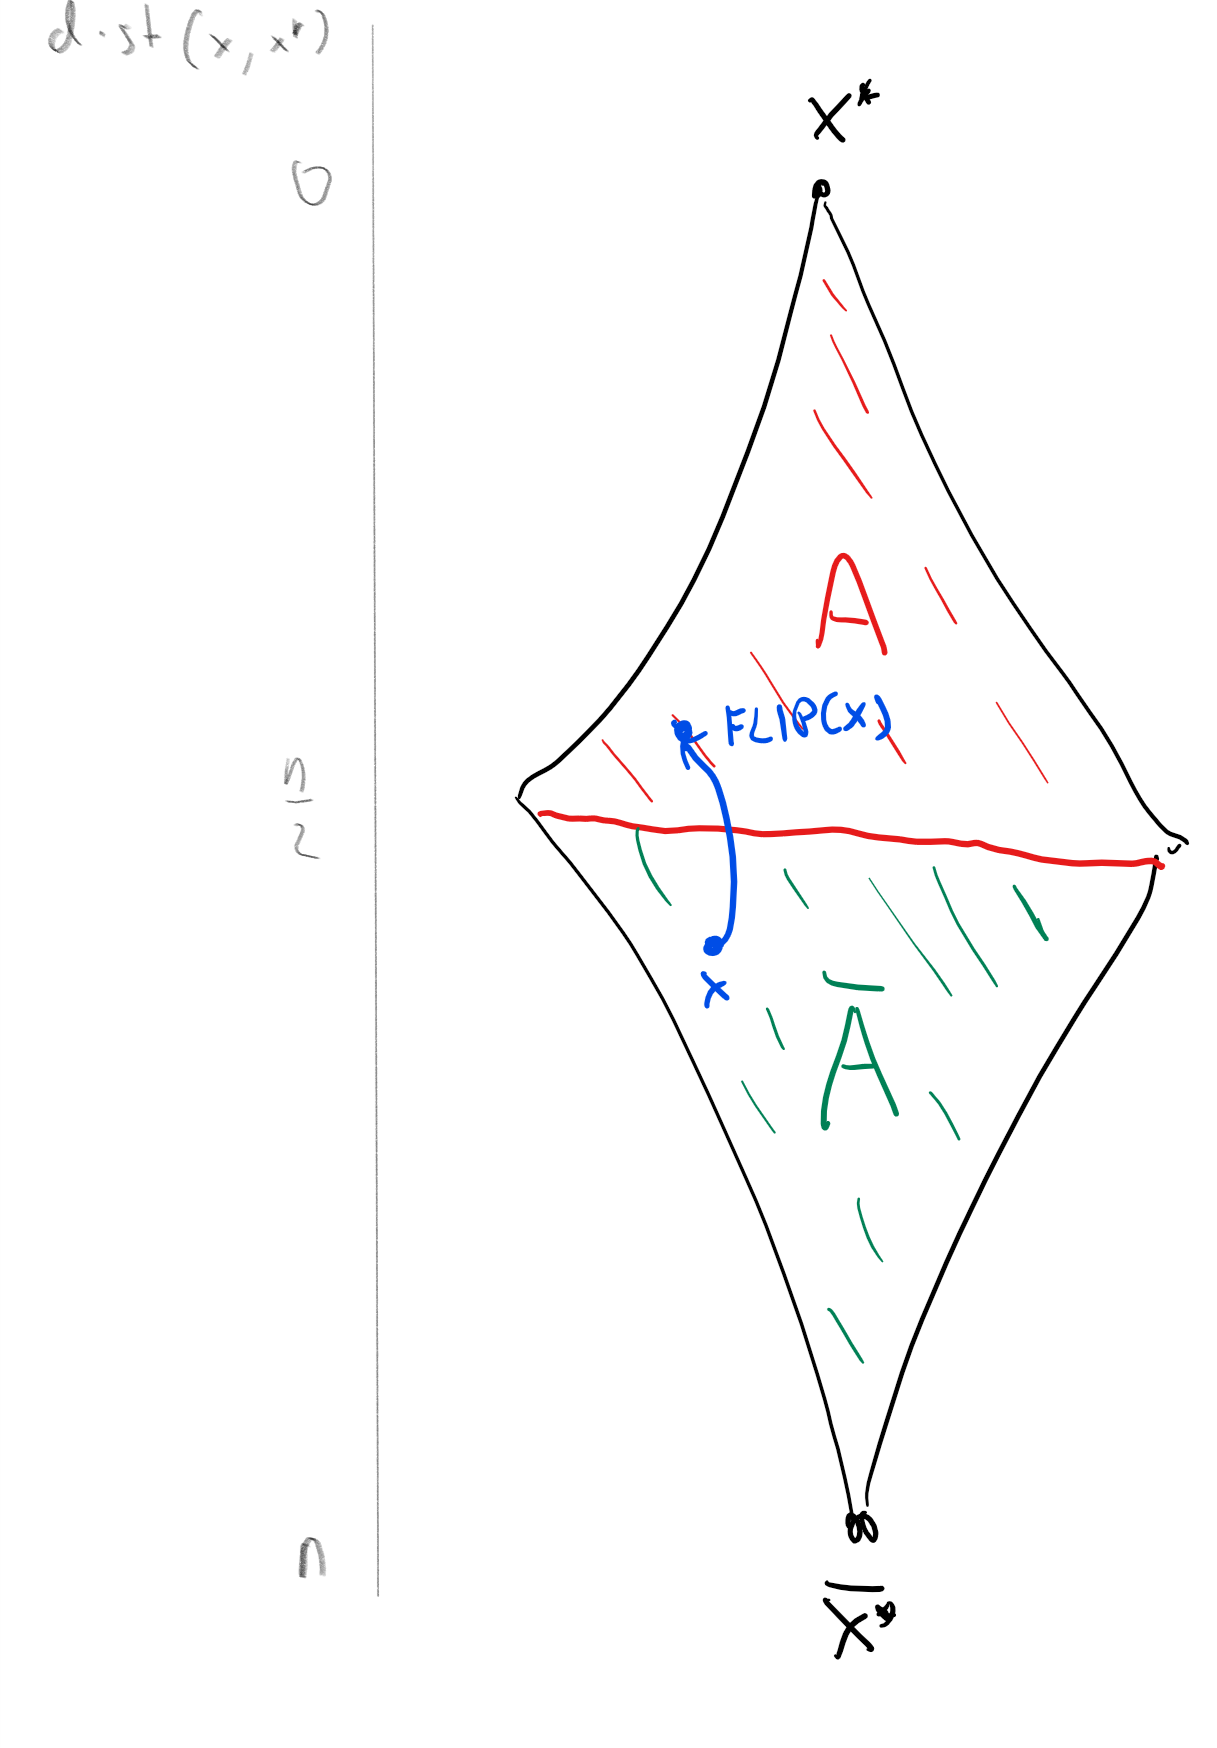
\includegraphics[width=\linewidth, height=1.5in, keepaspectratio]{../figure/flipaanalysis.png}
\caption{For every \(x^* \in \{0,1\}^n\), we can sort all strings in
\(\{0,1\}^n\) according to their distance from \(x^*\) (top to bottom in
the above figure), where we let
\(A = \{ x\in \{0,1\}^n \;|\; dist(x,x^* \leq n/2 \}\) be the ``top
half'' of strings. If we define
\(\ensuremath{\mathit{FLIP}}:\{0,1\}^n \rightarrow \{0,1\}\) to be the
map that ``flips'' the bits of a given string \(x\) then it maps every
\(x\in \overline{A}\) to an output
\(\ensuremath{\mathit{FLIP}}(x)\in A\) in a one-to-one way, and so it
demonstrates that \(|\overline{A}| \leq |A|\) which implies that
\(\Pr[A] \geq \Pr[\overline{A}]\) and hence \(\Pr[A] \geq 1/2\).}
\label{flipaanalysisfig}
\end{marginfigure}

\subsection{Bipartite matching.}\label{Bipartite-matching}

The \emph{matching} problem is one of the canonical optimization
problems, arising in all kinds of applications: matching residents with
hospitals, kidney donors with patients, flights with crews, and many
others. One prototypical variant is \emph{bipartite perfect matching}.
In this problem, we are given a bipartite graph \(G = (L\cup R,E)\)
which has \(2n\) vertices partitioned into \(n\)-sized sets \(L\) and
\(R\), where all edges have one endpoint in \(L\) and the other in
\(R\). The goal is to determine whether there is a \emph{perfect
matching}, a subset \(M \subseteq E\) of \(n\) disjoint edges. That is,
\(M\) matches every vertex in \(L\) to a unique vertex in \(R\).


\begin{marginfigure}
\centering
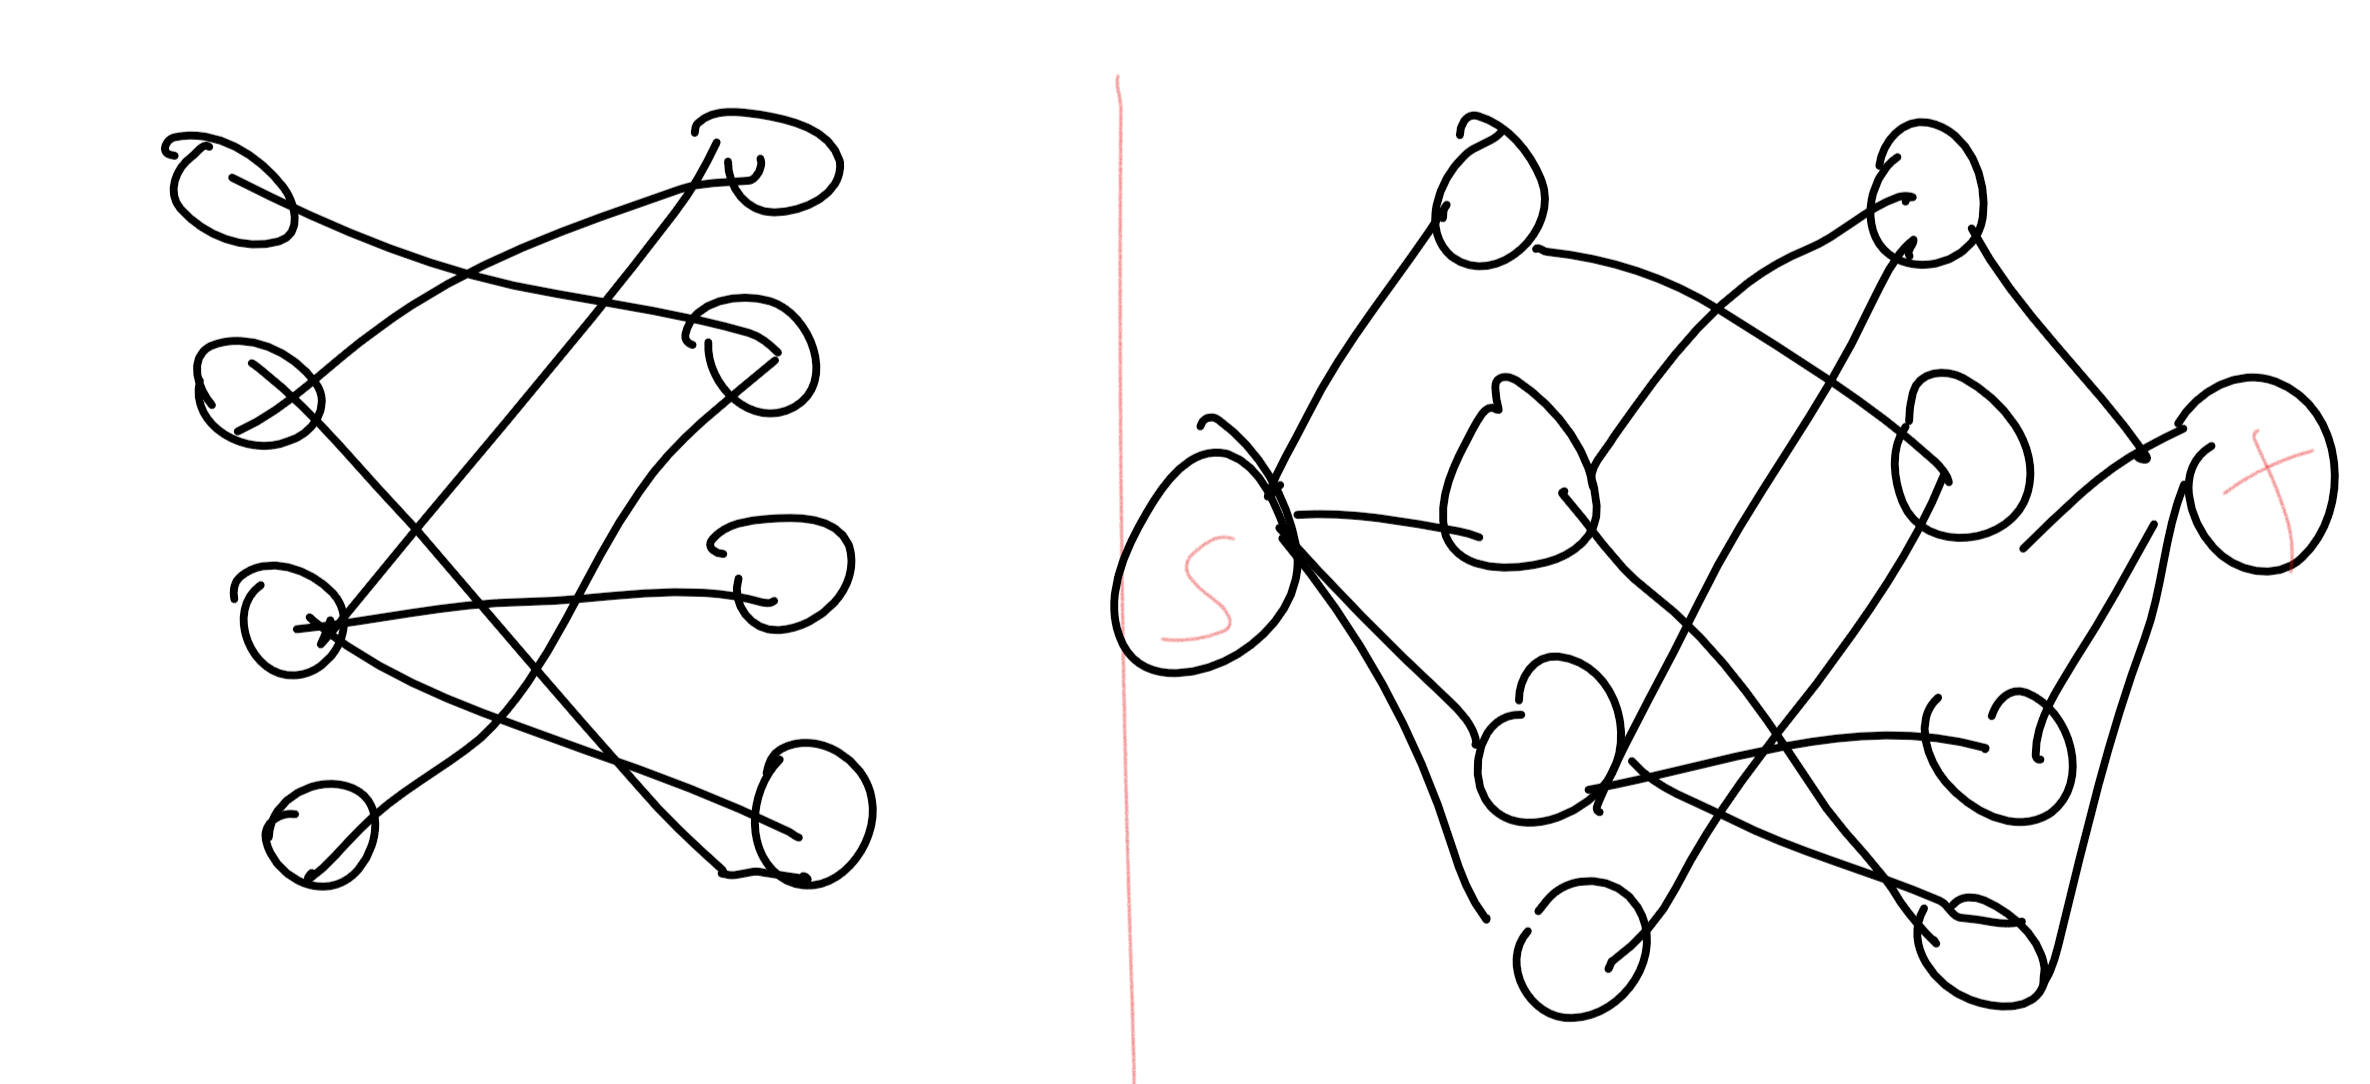
\includegraphics[width=\linewidth, height=1.5in, keepaspectratio]{../figure/matchingfig.png}
\caption{The bipartite matching problem in the graph \(G=(L\cup R,E)\)
can be reduced to the minimum \(s,t\) cut problem in the graph \(G'\)
obtained by adding vertices \(s,t\) to \(G\), connecting \(s\) with
\(L\) and connecting \(t\) with \(R\).}
\label{matchingfig}
\end{marginfigure}

The bipartite matching problem turns out to have a polynomial-time
algorithm, since we can reduce finding a matching in \(G\) to finding a
maximum flow (or equivalently, minimum cut) in a related graph \(G'\)
(see \cref{matchingfig}). However, we will see a different probabilistic
algorithm to determine whether a graph contains such a matching.

Let us label \(G\)'s vertices as \(L = \{ \ell_0,\ldots,\ell_{n-1} \}\)
and \(R = \{ r_0, \ldots, r_{n-1} \}\). A matching \(M\) corresponds to
a \emph{permutation} \(\pi \in S_n\) (i.e., one-to-one and onto function
\(\pi: [n] \rightarrow [n]\)) where for every \(i\in [n]\), we define
\(\pi(i)\) to be the unique \(j\) such that \(M\) contains the edge
\(\{ \ell_i ,r_j \}\). Define an \(n\times n\) matrix \(A=A(G)\) where
\(A_{i,j}=1\) if and only if the edge \(\{\ell_i,r_j\}\) is present and
\(A_{i,j}=0\) otherwise. The correspondence between matchings and
permutations implies the following claim:

\hypertarget{matchpolylem}{}
\begin{lemma}[Matching polynomial] \label[lemma]{matchpolylem}

Define \(P=P(G)\) to be the polynomial mapping \(\R^{n^2}\) to \(\R\)
where \[
P(x_{0,0},\ldots,x_{n-1,n-1}) = \sum_{\pi \in S_n} \left( \prod_{i=0}^{n-1} sign(\pi)A_{i,\pi(i)} \right) \prod_{i=0}^{n-1} x_{i,\pi(i)} \label{matchpolyeq}
\] Then \(G\) has a perfect matching if and only if \(P\) is not
identically zero. That is, \(G\) has a perfect matching if and only if
there exists some assignment \(x=(x_{i,j})_{i,j\in [n]} \in \R^{n^2}\)
such that \(P(x) \neq 0\).\footnote{The
  \href{https://goo.gl/ELnXhq}{sign} of a permutation
  \(\pi:[n] \rightarrow [n]\), denoted by \(sign(\pi)\), can be defined
  in several equivalent ways, one of which is that
  \(sign(\pi)=(-1)^{INV(\pi)}\) where
  \(\ensuremath{\mathit{INV}}(pi)=|\{(x,y) \in [n] \;|\; x<y \; \wedge \; \pi(x)>\pi(y)\}\)
  (i.e., \(\ensuremath{\mathit{INV}}(\pi)\) is the number of pairs of
  elements that are \emph{inverted} by \(\pi\)). The importance of the
  term \(sign(\pi)\) is that it makes \(P\) equal to the
  \emph{determinant} of the matrix \((x_{i,j})\) and hence efficiently
  computable.}

\end{lemma}

\begin{proof} \label[proof]{If-G-has-a-perfect-matchi}

If \(G\) has a perfect matching \(M^*\), then let \(\pi^*\) be the
permutation corresponding to \(M\) and let \(x^* \in \Z^{n^2}\) defined
as follows: \(x_{i,j}=1\) if \(j=\pi(i)\) and \(x_{i,j}=0\). Note that
for every \(\pi \neq \pi^*\), \(\prod_{i=0}^{n-1} x_{i,\pi(i)}=0\) but
\(\prod_{i=0}^{n-1} x^*_{i,\pi^*(i)}=1\). Hence \(P(x^*)\) will equal
\(\prod_{i=0}^{n-1} A_{i,\pi^*(i)}\). But since \(M^*\) is a perfect
matching in \(G\), \(\prod_{i=0}^{n-1} A_{i,\pi^*(i)} = 1\).

On the other hand, suppose that \(P\) is not identically zero. By
\eqref{matchpolyeq}, this means that at least one of the terms
\(\prod_{i=0}^{n-1}A_{i,\pi(i)}\) is not equal to zero. But then this
permutation \(\pi\) must be a perfect matching in \(G\).

\end{proof}

As we've seen before, for every \(x \in \R^{n^2}\), we can compute
\(P(x)\) by simply computing the \emph{determinant} of the matrix
\(A(x)\), which is obtained by replacing \(A_{i,j}\) with
\(A_{i,j}x_{i,j}\). This reduces testing perfect matching to the
\emph{zero testing} problem for polynomials: given some polynomial
\(P(\cdot)\), test whether \(P\) is identically zero or not. The
intuition behind our randomized algorithm for zero testing is the
following:

\begin{quote}
\emph{If a polynomial is not identically zero, then it can't have ``too
many'' roots.}
\end{quote}


\begin{marginfigure}
\centering
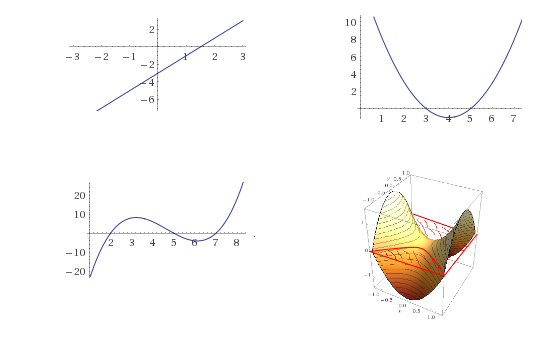
\includegraphics[width=\linewidth, height=1.5in, keepaspectratio]{../figure/curves.png}
\caption{A degree \(d\) curve in one variable can have at most \(d\)
roots. In higher dimensions, a \(n\)-variate degree-\(d\) polynomial can
have an infinite number roots though the set of roots will be an \(n-1\)
dimensional surface. Over a finite field \(\mathbb{F}\), an
\(n\)-variate degree \(d\) polynomial has at most
\(d|\mathbb{F}|^{n-1}\) roots.}
\label{curvesfig}
\end{marginfigure}

This intuition sort of makes sense. For one variable polynomials, we
know that a nonzero linear function has at most one root, a quadratic
function (e.g., a parabola) has at most two roots, and generally a
degree \(d\) equation has at most \(d\) roots. While in more than one
variable there can be an infinite number of roots (e.g., the polynomial
\(x_0+y_0\) vanishes on the line \(y=-x\)) it is still the case that the
set of roots is very ``small'' compared to the set of all inputs. For
example, the root of a bivariate polynomial form a curve, the roots of a
three-variable polynomial form a surface, and more generally the roots
of an \(n\)-variable polynomial are a space of dimension \(n-1\).

This intuition leads to the following simple randomized algorithm:

\begin{quote}
\emph{To decide if \(P\) is identically zero, choose a ``random'' input
\(x\) and check if \(P(x)\neq 0\).}
\end{quote}

This makes sense: if there are only ``few'' roots, then we expect that
with high probability the random input \(x\) is not going to be one of
those roots. However, to transform this into an actual algorithm, we
need to make both the intuition and the notion of a ``random'' input
precise. Choosing a random real number is quite problematic, especially
when you have only a finite number of coins at your disposal, and so we
start by reducing the task to a finite setting. We will use the
following result

\hypertarget{szlem}{}
\begin{theorem}[Schwartz–Zippel lemma] \label[theorem]{szlem}

For every integer \(q\), and polynomial \(P:\R^n \rightarrow \R\) with
integer coefficients. If \(P\) has degree at most \(d\) and is not
identically zero, then it has at most \(dq^{n-1}\) roots in the set
\([q]^n = \{ (x_0,\ldots,x_{n-1}) : x_i \in \{0,\ldots,q-1\} \}\).

\end{theorem}

We omit the (not too complicated) proof of \cref{szlem}. We remark that
it holds not just over the real numbers but over any field as well.
Since the matching polynomial \(P\) of \cref{matchpolylem} has degree at
most \(n\), \cref{szlem} leads directly to a simple algorithm for
testing if it is nonzero:

\begin{quote} \label[quote]{Algorithm-Perfect-Matchin}

\textbf{Algorithm Perfect-Matching:}

\textbf{Input:} Bipartite graph \(G\) on \(2n\) vertices
\(\{ \ell_0,\ldots,\ell_{n-1} , r_0,\ldots,r_{n-1} \}\).

\textbf{Operation:}

\begin{enumerate}
\def\labelenumi{\arabic{enumi}.}
\item
  For every \(i,j \in [n]\), choose \(x_{i,j}\) independently at random
  from \([2n]=\{0,\ldots 2n-1\}\).
\item
  Compute the determinant of the matrix \(A(x)\) whose \((i,j)^{th}\)
  entry equals \(x_{i,j}\) if the edge \(\{\ell_i,r_j\}\) is present and
  \(0\) otherwise.
\item
  Output \texttt{no perfect matching} if this determinant is zero, and
  output \texttt{perfect matching} otherwise.
\end{enumerate}

\end{quote}

This algorithm can be improved further (e.g., see \cref{matchingmodex}).
While it is not necessarily faster than the cut-based algorithms for
perfect matching, it does have some advantages. In particular, it is
more amenable for parallelization. (However, it also has the significant
disadvantage that it does not produce a matching but only states that
one exists.) The Schwartz--Zippel Lemma, and the associated zero testing
algorithm for polynomials, is widely used across computer science,
including in several settings where we have no known deterministic
algorithm matching their performance.

\begin{recap} \label[recap]{Using-concentration-resul}

\begin{itemize}
\item
  Using concentration results, we can \emph{amplify} in polynomial time
  the success probability of a probabilistic algorithm from a mere
  \(1/p(n)\) to \(1-2^{-q(n)}\) for every polynomials \(p\) and \(q\).
\item
  There are several randomized algorithms that are better in various
  senses (e.g., simpler, faster, or other advantages) than the best
  known deterministic algorithm for the same problem.
\end{itemize}

\end{recap}

\section{Exercises}\label{Exercises}

\hypertarget{cutalgorithmamplificationlemex}{}
\begin{exercise}[Amplification for max cut] \label[exercise]{cutalgorithmamplificationlemex}

Prove \cref{cutalgorithmamplificationlem}

\end{exercise}

\hypertarget{maxcutex}{}
\begin{exercise}[Deterministic max cut algorithm] \label[exercise]{maxcutex}

\footnote{TODO: add exercise to give a deterministic max cut algorithm
  that gives \(m/2\) edges. Talk about greedy approach.}

\end{exercise}

\hypertarget{coindistex}{}
\begin{exercise}[Simulating distributions using coins] \label[exercise]{coindistex}

Our model for probability involves tossing \(n\) coins, but sometimes
algorithm require sampling from other distributions, such as selecting a
uniform number in \(\{0,\ldots,M-1\}\) for some \(M\). Fortunately, we
can simulate this with an exponentially small probability of error:
prove that for every \(M\), if \(n>k\lceil \log M \rceil\), then there
is a function
\(F:\{0,1\}^n \rightarrow \{0,\ldots,M-1\} \cup \{ \bot \}\) such that
\textbf{(1)} The probability that \(F(x)=\bot\) is at most \(2^{-k}\)
and \textbf{(2)} the distribution of \(F(x)\) conditioned on
\(F(x) \neq \bot\) is equal to the uniform distribution over
\(\{0,\ldots,M-1\}\).\footnote{\textbf{Hint:} Think of
  \(x\in \{0,1\}^n\) as choosing \(k\) numbers
  \(y_1,\ldots,y_k \in \{0,\ldots, 2^{\lceil \log M \rceil}-1 \}\).
  Output the first such number that is in \(\{0,\ldots,M-1\}\). }

\end{exercise}

\hypertarget{walksatex}{}
\begin{exercise}[Better walksat analysis] \label[exercise]{walksatex}

\begin{enumerate}
\def\labelenumi{\arabic{enumi}.}
\tightlist
\item
  Prove that for every \(\epsilon>0\), if \(n\) is large enough then for
  every \(x^*\in \{0,1\}^n\)
  \(\Pr_{x \sim \{0,1\}^n}[ \Delta(x,x^*) \leq n/3 ] \leq 2^{-(1-H(1/3)-\epsilon)n}\)
  where \(H(p)=p\log(1/p) + (1-p)\log(1/(1-p))\) is the same function as
  in \cref{entropybinomex}.\\
\item
  Prove that \(2^{1-H(1/4)+(1/4) \log 3}=(3/2)\).
\item
  Use the above to prove that for every \(\delta>0\) and large enough
  \(n\), if we set \(T=1000\cdot (3/2+\delta)^n\) and \(S=n/4\) in the
  WalkSAT algorithm then for every satisfiable 3CNF \(\varphi\), the
  probability that we output \texttt{unsatisfiable} is at most
  \(1/2\).\\
\end{enumerate}

\end{exercise}

\hypertarget{matchingmodex}{}
\begin{exercise}[Faster bipartite matching (challenge)] \label[exercise]{matchingmodex}

(to be completed: improve the matching algorithm by working modulo a
prime)

\end{exercise}

\section{Bibliographical notes}\label{Bibliographical-notes}

The books of Motwani and Raghavan \cite{motwani1995randomized} and
Mitzenmacher and Upfal \cite{mitzenmacher2017probability} are two
excellent resources for randomized algorithms. Some of the history of
the discovery of Monte Carlo algorithm is covered
\href{http://permalink.lanl.gov/object/tr?what=info:lanl-repo/lareport/LA-UR-88-9068}{here}.

\section{Acknowledgements}\label{Acknowledgements}
